\documentclass[11pt,letterpaper]{article}
\usepackage{pdfpages}
\usepackage{fancyhdr}
\usepackage[colorlinks=true, urlcolor=blue, linkcolor=blue]{hyperref}
\usepackage{graphicx}
\usepackage[top=1.4in, left=0.5in, right=0.5in, bottom=0.8in]{geometry}
\usepackage[T1]{fontenc}
\usepackage{helvet}
\usepackage{fontawesome}
\pagestyle{fancy}
\renewcommand{\headrulewidth}{0pt}
\renewcommand{\footrulewidth}{0pt}
\setlength{\parindent}{0em}
\setlength{\parskip}{1em}


\fancyfoot[C]{\setlength{\unitlength}{1in}\begin{picture}(5,0)\put(-1.8,-1){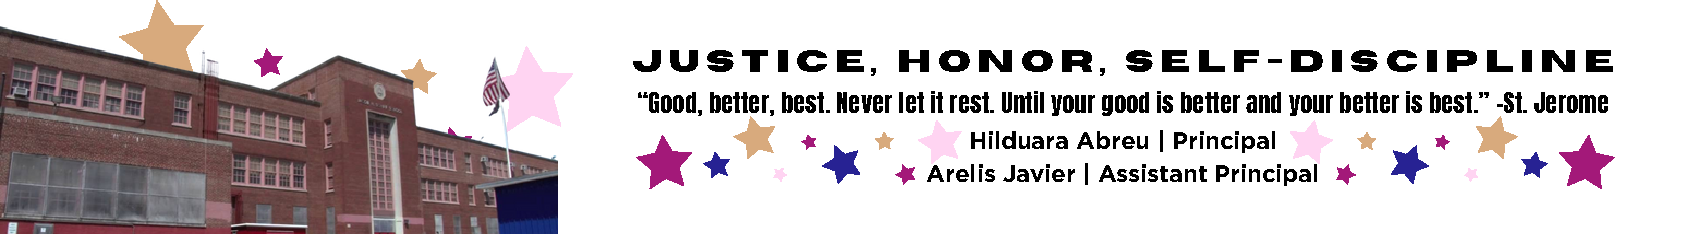
\includegraphics[width=8.8in,height=1.3in]{logo-1}}\end{picture}}
\fancyhead[C]{\setlength{\unitlength}{1in}\begin{picture}(5,0)\put(-1.9,-1){
\includegraphics[width=8.9in,height=1.3in]{logo-2}}\end{picture}}

\pagenumbering{gobble}
\addtolength{\evensidemargin}{-2in}
\addtolength{\topmargin}{-0.5in}
\addtolength{\textwidth}{0in}
%%%%%%%%%%%%%%%%%%%%%%%%%%%%%%%%%%%%%%%%%%%%%%%%%%%%%%%%%%%%%%%%%%

\begin{document}
\vspace*{0.5in}
Date: \href{https://www.ps192.org/}{October, 2023} 

\textbf{Subject: Citywide Behavioral Expectations Lessons Assurance Form}

All classroom teachers have been provided with a digital copy of the Citywide Behavioral Expectations to Support Student Learning. (click the link .)

Please make sure that your review the disciplinary protocols for your specific grade during the month of September. In addition, after a careful review and discussion with your students, upload the grade specific section on your google classroom to be used as a reference throughout the school year. All teachers must be familiar with disciplinary protocols for their specific grade levels. 

No later than Friday, September 29, 2023 , all classroom and homeroom teachers will review relevant pages with their students. Teachers in departmentalized grades should review specified pages during a period in which they meet with their homeroom class that day.

All teachers must sign off that they have reviewed this material with their students. Students in Grades 2-5 must indicate in writing that they have participated in the lesson. Follow-up lessons should be planned as needed during the class SEL block.

Please return the bottom portion of this page (with Grade 2-5 student sign-offs) to Assistant Principal Arelis Javier  by close of day on Monday, October 2, 2023. 
\par\rule{\textwidth}{0.5pt}
\par
\begin{center}
\textbf{Citywide Behavioral Expectations Lessons}
\end{center}
Teacher:\line(1,0){150}\hspace{20em}Class:\line(1,0){75}
\begin{itemize}
	\item[\faSquareO] I have reviewed the specified pages of the DOE Discipline
	 Booklet with my  students.
	\item[\faSquareO] I have attached the student sign-off sheet dated\line(1,0)
	{75}(date of lesson).
\end{itemize}

\vspace{10mm}

\begin{center}
\noindent\begin{tabular}{ll}
\makebox[2.5in]{\hrulefill} & \makebox[2.5in]{\hrulefill}\\
Teacher's Signature & Date\\[8ex]% adds space between the two sets of signatures
\end{tabular}
\end{center}



\end{document}
